\section{Nestrukturovaná a částečně strukturovaná data. Porovnávání vzorů, indexování a vyhledávání dokumentů, extrakce informací a web scraping}

\subsection*{Základní vymezení}

Data lze podle míry strukturovanosti rozdělit na:
\begin{itemize}
    \item \textbf{strukturovaná data} -- mají pevné schéma, typicky relační tabulky v databázi;
    \item \textbf{semistrukturovaná data} -- mají vnitřní strukturu, ale ta nemusí být pevně tabulková,
    například XML, JSON, HTML nebo logy;
    \item \textbf{nestrukturovaná data} -- nemají pevnou tabulkovou strukturu, například volný text,
    dokumenty, PDF, e-maily, obrázky, audio, video nebo webové stránky.
\end{itemize}

\paragraph{Důležitá poznámka.}
Text se často označuje jako nestrukturovaný, ale není úplně bez struktury. Přirozený jazyk má slova,
věty, gramatiku, syntax, morfologii a významové vztahy. Pro databázový systém ale obvykle nejde o předem
dané řádky a sloupce, a proto se text řadí mezi nestrukturovaná nebo slabě strukturovaná data.

\subsection*{Semistrukturovaná data}

Semistrukturovaná data mají značky, klíče nebo hierarchii, které umožňují obsah strojově zpracovat.
Prakticky je důležité nepřistupovat k nim jako k obyčejnému řetězci, pokud existuje parser pro daný formát:
u XML a HTML je bezpečnější pracovat se stromem dokumentu, u JSONu s objekty a poli.

\subsubsection*{XML}

XML je značkovací jazyk se stromovou strukturou. Data jsou tvořena elementy, atributy a textovým obsahem.

Příklad:
\[
\texttt{<book id="1"><title>Data Mining</title><price>39.90</price></book>}
\]

Vlastnosti XML:
\begin{itemize}
    \item stromová struktura,
    \item značky oddělují jednotlivé části dokumentu,
    \item možnost validace přes DTD nebo XML Schema,
    \item vhodné pro dokumenty, konfigurace a výměnu dat.
\end{itemize}

Pro dotazování nad XML se používají například:
\begin{itemize}
    \item \textbf{XPath} -- výběr uzlů ve stromu,
    \item \textbf{XQuery} -- dotazovací jazyk pro XML dokumenty.
\end{itemize}

\subsubsection*{JSON}

JSON je lehčí formát často používaný ve webových API a dokumentových databázích.

Příklad:
\[
\texttt{\{"id": 1, "title": "Data Mining", "price": 39.90\}}
\]

Vlastnosti JSON:
\begin{itemize}
    \item objekt je množina dvojic klíč--hodnota,
    \item podporuje pole, čísla, řetězce, logické hodnoty a vnořené objekty,
    \item je přirozeně použitelný v JavaScriptu,
    \item používá se v REST API, logování, konfiguracích a NoSQL databázích.
\end{itemize}

Dokumentové databáze, například MongoDB nebo CouchDB, ukládají záznamy právě jako dokumenty podobné JSONu.
Výhodou je flexibilita schématu, nevýhodou slabší kontrola integrity než u dobře navrženého relačního modelu.

\subsubsection*{HTML a DOM}

HTML je značkovací jazyk webových stránek. Pro web scraping je důležitý model DOM:
\[
\text{HTML dokument} \rightarrow \text{DOM strom}.
\]

DOM strom umožňuje vybírat prvky stránky pomocí:
\begin{itemize}
    \item CSS selektorů,
    \item XPath výrazů,
    \item navigace přes rodiče, potomky a sourozence uzlů.
\end{itemize}

Například CSS selektor:
\[
\texttt{div.product span.price}
\]
vybere cenu uvnitř elementu \texttt{span} s třídou \texttt{price}, který je uvnitř produktu.

\begin{figure}[htbp]
  \centering
  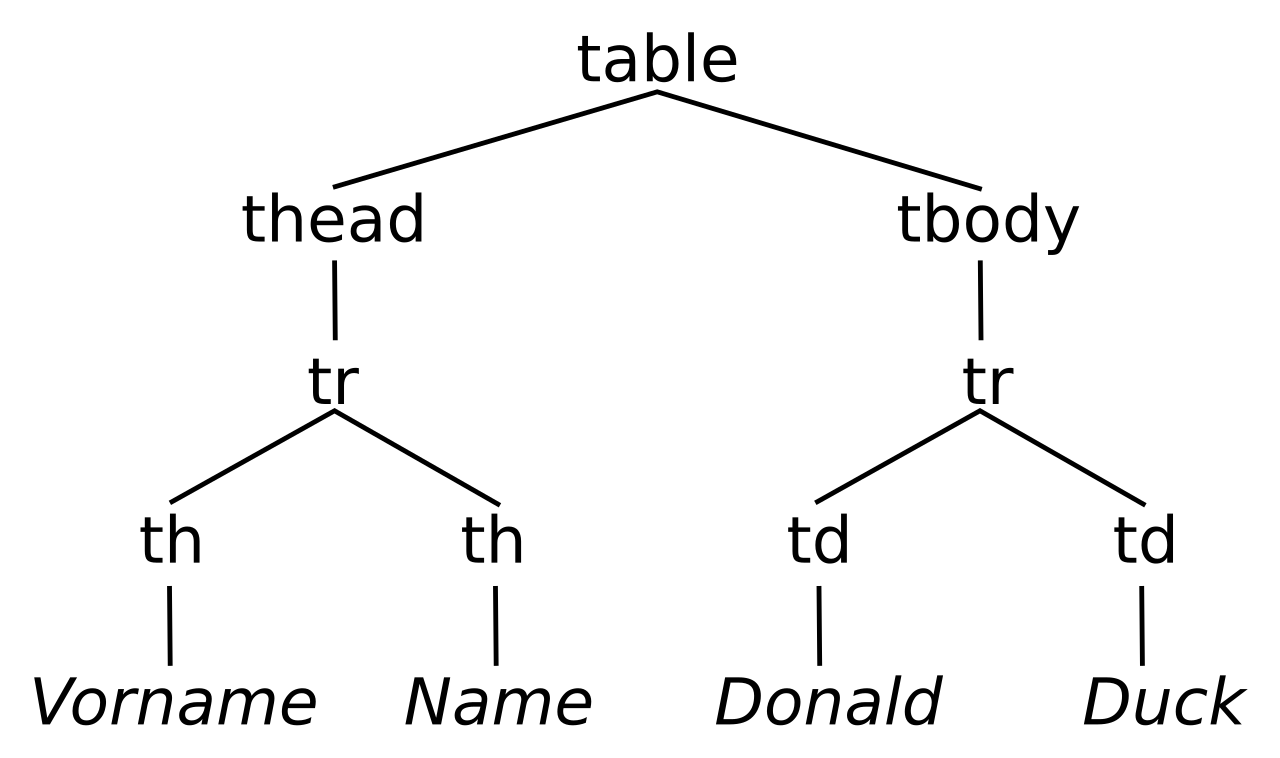
\includegraphics[width=0.70\linewidth]{assets/images/nestrukturovana-data/dom-tree.png}
  \caption[DOM strom HTML dokumentu]{Příklad DOM stromu. Popis obrázku: elementy HTML tabulky tvoří
  hierarchii rodičů a potomků, nad kterou lze vybírat uzly pomocí CSS selektorů, XPath nebo navigace ve
  stromu. Zdroj obrázku: Molily, SVG Marlus Gancher,
  \href{https://commons.wikimedia.org/wiki/File:DOM\_Beispielbaum.svg}{Wikimedia Commons}, public domain.}
  \label{fig:q17-dom-tree}
\end{figure}

\subsection*{Porovnávání vzorů}

Porovnávání vzorů znamená hledání částí dat, které odpovídají určitému předpisu. Může jít o:
\begin{itemize}
    \item přesné porovnání řetězců,
    \item regulární výrazy,
    \item přibližné porovnání řetězců,
    \item podobnost dokumentů nebo embeddingů.
\end{itemize}

\subsection*{Regulární výrazy}

Regulární výraz je formální textový vzor, který umožňuje vyhledávat, validovat, extrahovat nebo nahrazovat
části textu.

Použití:
\begin{itemize}
    \item validace e-mailu, telefonu, PSČ nebo identifikátoru,
    \item extrakce dat, měnových částek, IP adres nebo kódů,
    \item čištění logů,
    \item normalizace textu,
    \item rychlá extrakce jednoduchých entit.
\end{itemize}

\subsubsection*{Základní prvky regulárních výrazů}

\begin{itemize}
    \item \textbf{literál} -- obyčejný znak, například \texttt{a};
    \item \textbf{metaznak} -- znak se speciálním významem;
    \item \textbf{escape} -- zrušení speciálního významu metaznaku;
    \item \textbf{znaková třída} -- množina povolených znaků;
    \item \textbf{kvantifikátor} -- počet opakování;
    \item \textbf{skupina} -- část vzoru uzavřená v závorkách;
    \item \textbf{alternativa} -- výběr jedné z možností.
\end{itemize}

Příklady:
\[
\texttt{\textbackslash d}
\quad
\text{číslice},
\qquad
\texttt{\textbackslash w}
\quad
\text{slovní znak},
\qquad
\texttt{\textbackslash s}
\quad
\text{bílý znak}.
\]

Kvantifikátory:
\[
\texttt{*}
\quad
\text{0 nebo více výskytů},
\qquad
\texttt{+}
\quad
\text{1 nebo více výskytů},
\qquad
\texttt{?}
\quad
\text{0 nebo 1 výskyt}.
\]

Začátek a konec řetězce:
\[
\texttt{\string^}
\quad
\text{začátek},
\qquad
\texttt{\$}
\quad
\text{konec}.
\]

\subsubsection*{Příklad extrakce částky}

Chceme najít částky typu:
\[
\texttt{23 MEUR},\quad \texttt{500 EUR},\quad \texttt{17 KEUR}.
\]

Regex:
\[
\texttt{(\textbackslash d+)\textbackslash s*(MEUR|KEUR|EUR)}
\]

Význam:
\begin{itemize}
    \item \texttt{(\textbackslash d+)} -- jedna nebo více číslic, první zachycená skupina;
    \item \texttt{\textbackslash s*} -- libovolný počet mezer;
    \item \texttt{(MEUR|KEUR|EUR)} -- jedna z měnových jednotek.
\end{itemize}

\subsubsection*{Lookaround}

Lookaround umožňuje kontrolovat okolí nalezeného výrazu, aniž by se toto okolí stalo součástí výsledku.

\begin{itemize}
    \item \textbf{positive lookahead}: výraz musí následovat;
    \item \textbf{negative lookahead}: výraz nesmí následovat;
    \item \textbf{positive lookbehind}: výraz musí předcházet;
    \item \textbf{negative lookbehind}: výraz nesmí předcházet.
\end{itemize}

Například chceme najít číslo jen tehdy, pokud za ním následuje \texttt{EUR}:
\[
\texttt{\textbackslash d+(?=\textbackslash s*EUR)}
\]

\subsubsection*{Silné a slabé stránky regexů}

Výhody:
\begin{itemize}
    \item rychlé a přesné pro formální vzory,
    \item dobré pro kódy, data, měny, ID, e-maily, logy,
    \item jednoduché nasazení bez trénovacích dat.
\end{itemize}

Nevýhody:
\begin{itemize}
    \item špatně zachycují význam a kontext,
    \item pro přirozený jazyk bývají křehké,
    \item složité regexy jsou málo čitelné,
    \item při změně formátu dat se snadno rozbijí.
\end{itemize}

\paragraph{Typická chyba.}
Regex je vhodný pro jednoduchý textový vzor, ale není dobrý obecný parser HTML nebo XML. U webových stránek je
spolehlivější nejprve vytvořit DOM strom a až potom vybírat konkrétní elementy.

\subsection*{Přibližné porovnávání řetězců}

Přibližné porovnávání řetězců řeší situace, kdy texty nejsou totožné, ale jsou podobné:
\[
\texttt{international}
\quad
\text{vs.}
\quad
\texttt{internationalization}.
\]

Typické míry:
\begin{itemize}
    \item \textbf{Hammingova vzdálenost} -- počet rozdílných znaků na stejných pozicích;
    \item \textbf{Levenshteinova vzdálenost} -- minimální počet vložení, smazání a nahrazení;
    \item \textbf{Jaro-Winkler} -- vhodné pro jména a krátké řetězce;
    \item \textbf{nejdelší společná podposloupnost} -- délka nejdelší posloupnosti zachované v obou textech.
\end{itemize}

Levenshteinova vzdálenost:
\[
d(i,j)=
\min
\begin{cases}
d(i-1,j)+1,\\
d(i,j-1)+1,\\
d(i-1,j-1)+I(x_i\neq y_j).
\end{cases}
\]

Použití:
\begin{itemize}
    \item deduplikace záznamů,
    \item fuzzy matching jmen,
    \item opravy překlepů,
    \item propojení dat z různých zdrojů.
\end{itemize}

\subsection*{Information Retrieval}

Information Retrieval, zkráceně IR, je oblast zabývající se vyhledáváním relevantních dokumentů v kolekci
textů. Uživatel formuluje informační potřebu jako dotaz a systém vrací dokumenty nebo pasáže, které dotazu
odpovídají.

\paragraph{Základní architektura IR systému.}
\[
\begin{aligned}
\text{kolekce dokumentů}
&\rightarrow
\text{indexer}
\rightarrow
\text{index},\\
\text{uživatelský dotaz}
&\rightarrow
\text{query operations}
\rightarrow
\text{spustitelný dotaz},\\
\text{index + dotaz}
&\rightarrow
\text{retrieval system}
\rightarrow
\text{seřazené dokumenty}.
\end{aligned}
\]

\begin{figure}[htbp]
  \centering
  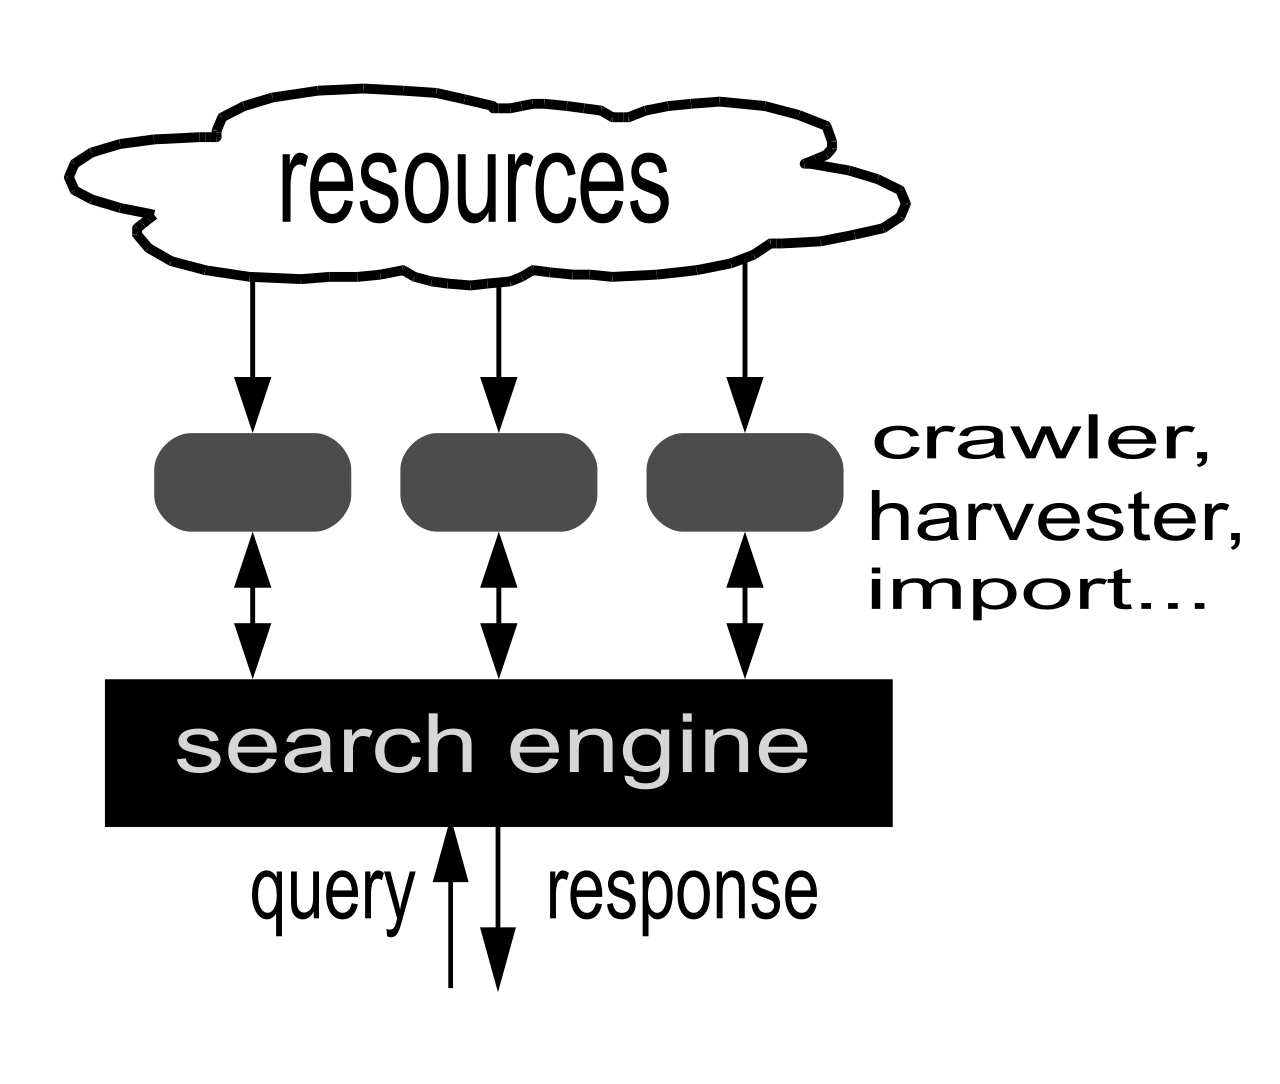
\includegraphics[width=0.66\linewidth]{assets/images/nestrukturovana-data/search-engine-concept.png}
  \caption[Koncept vyhledávače]{Zjednodušený koncept vyhledávače. Popis obrázku: crawler nebo harvester
  získává zdroje, vyhledávač nad nimi vytváří index a uživatel posílá dotaz, na který systém vrací odpověď
  nebo seřazené výsledky. Zdroj obrázku: Jakob Voss,
  \href{https://commons.wikimedia.org/wiki/File:Search-engine-diagram-en.svg}{Wikimedia Commons}, licence
  CC BY-SA 4.0.}
  \label{fig:q17-search-engine}
\end{figure}

\subsection*{Typy dotazů}

V IR se používají různé typy dotazů:
\begin{itemize}
    \item \textbf{keyword query} -- dotaz tvořený klíčovým slovem;
    \item \textbf{boolean query} -- dotaz pomocí AND, OR, NOT;
    \item \textbf{phrase query} -- přesná fráze, například \texttt{"data mining"};
    \item \textbf{proximity query} -- slova musí být blízko sebe;
    \item \textbf{full document query} -- dotazem je celý dokument;
    \item \textbf{natural language question} -- dotaz ve formě přirozené otázky.
\end{itemize}

Příklad:
\[
\texttt{cat AND dog}
\]
vrátí dokumenty obsahující oba termy.

\[
\texttt{cat AND NOT dog}
\]
vrátí dokumenty s termem \texttt{cat}, ale bez termu \texttt{dog}.

\subsection*{Předzpracování dokumentů pro vyhledávání}

Před vytvořením indexu se dokumenty obvykle převádějí do vhodné reprezentace.

Typický postup:
\begin{enumerate}
    \item získání dokumentů,
    \item extrakce textu z HTML, PDF, Wordu nebo skenů,
    \item OCR u skenovaných dokumentů,
    \item tokenizace,
    \item normalizace velikosti písmen,
    \item odstranění interpunkce nebo šumu,
    \item odstranění stop slov,
    \item stemming nebo lemmatizace,
    \item vytvoření termů, n-gramů nebo embeddingů,
    \item vytvoření indexu.
\end{enumerate}

\paragraph{Stop slova.}
Stop slova jsou častá slova s nízkou informační hodnotou, například \uv{a}, \uv{the}, \uv{of}.
Jejich odstranění může zmenšit index, ale u některých dotazů může škodit.

\paragraph{Stemming vs. lemmatizace.}
Stemming hrubě zkracuje slovo na kmen:
\[
\text{running},\ \text{runner},\ \text{runs}
\rightarrow
\text{run}.
\]

Lemmatizace převádí slovo na slovníkový tvar:
\[
\text{šel},\ \text{šla},\ \text{šli}
\rightarrow
\text{jít}.
\]

U češtiny je kvůli bohaté morfologii často vhodnější lemmatizace než jednoduchý stemming.

\subsection*{Document-term matice}

Po tokenizaci lze kolekci dokumentů reprezentovat jako document-term matici:
\[
X=(x_{ij}),
\]
kde:
\begin{itemize}
    \item řádky odpovídají dokumentům,
    \item sloupce termům,
    \item $x_{ij}$ je váha termu $j$ v dokumentu $i$.
\end{itemize}

Jednoduchá hodnota:
\[
x_{ij}=f_{ij},
\]
kde $f_{ij}$ je počet výskytů termu $j$ v dokumentu $i$.

\subsection*{Inverted index}

Pro rychlé vyhledávání se nepoužívá přímo celá document-term matice, ale \textbf{inverted index}.

Inverted index ukládá pro každý term seznam dokumentů, ve kterých se term vyskytuje:
\[
\text{term}
\rightarrow
\{(docID, frequency, positions)\}.
\]

Příklad:
\[
\texttt{cat}
\rightarrow
\{(d_1,2,[3,17]),(d_4,1,[8]),(d_9,5,[1,6,9,13,20])\}.
\]

Výhody:
\begin{itemize}
    \item rychlé vyhledávání dokumentů obsahujících term,
    \item možnost počítat skóre relevance,
    \item možnost podporovat frázové a proximity dotazy pomocí pozic termů.
\end{itemize}

\paragraph{Proč je index obrácený.}
Přímá reprezentace říká \uv{dokument $\rightarrow$ termy}. Vyhledávání ale typicky začíná termem v dotazu,
proto je efektivnější mít mapování \uv{term $\rightarrow$ dokumenty}. U velkých kolekcí se navíc posting listy
komprimují a při booleovském dotazu se nad nimi počítají průniky, sjednocení nebo rozdíly.

\subsection*{Booleovský model vyhledávání}

Booleovský model reprezentuje dokumenty jako množiny termů. Dotaz je logický výraz.

Operátory:
\[
AND,\quad OR,\quad NOT.
\]

Dokument je buď relevantní, nebo nerelevantní:
\[
rel(d,q)\in\{0,1\}.
\]

Výhody:
\begin{itemize}
    \item jednoduchý,
    \item přesný pro formální dotazy,
    \item dobře srozumitelný pro experty.
\end{itemize}

Nevýhody:
\begin{itemize}
    \item nepracuje dobře se stupněm relevance,
    \item neumí přirozeně řadit výsledky,
    \item nebere v úvahu frekvenci termů,
    \item AND může být příliš přísné a OR příliš široké.
\end{itemize}

\subsection*{Vektorový model vyhledávání}

Vektorový model reprezentuje dokument i dotaz jako vektory v prostoru termů:
\[
d_i=(w_{i1},w_{i2},\ldots,w_{ip}),
\]
\[
q=(w_{q1},w_{q2},\ldots,w_{qp}).
\]

Relevance dokumentu k dotazu se měří podobností vektorů. Nejčastěji kosinovou podobností:
\[
\cos(d_i,q)
=
\frac{d_i^\top q}
{\|d_i\|\|q\|}.
\]

Výsledek:
\begin{itemize}
    \item dokumenty nejsou jen relevantní/nerelevantní,
    \item dokumenty lze seřadit podle podobnosti s dotazem,
    \item model přirozeně využívá váhy termů.
\end{itemize}

\subsection*{TF-IDF}

TF-IDF je klasická váha termu v dokumentu. Kombinuje:
\begin{itemize}
    \item \textbf{TF} -- term frequency, tedy četnost termu v dokumentu;
    \item \textbf{IDF} -- inverse document frequency, tedy vzácnost termu v celé kolekci.
\end{itemize}

Term frequency:
\[
tf_{ij}=f_{ij}.
\]

Document frequency:
\[
df_j
=
|\{d_i:t_j\in d_i\}|.
\]

Inverse document frequency:
\[
idf_j
=
\log\left(\frac{N}{df_j}\right),
\]
kde $N$ je počet dokumentů v kolekci.

TF-IDF:
\[
w_{ij}
=
tf_{ij}\cdot idf_j.
\]

\paragraph{Intuice.}
Term je důležitý, pokud se často vyskytuje v daném dokumentu, ale není běžný ve všech dokumentech.

Slovo jako \uv{the} má vysokou četnost, ale nízké IDF. Specializovaný term může mít vysoké IDF.

\subsection*{BM25}

BM25 je modernější pravděpodobnostní skórovací funkce často používaná ve vyhledávačích.

Pro dotaz $q$ a dokument $d$:
\[
\begin{aligned}
score(d,q)
&=
\sum_{t\in q}
idf(t)
\frac{
f(t,d)(k_1+1)
}{
f(t,d)+k_1\left(1-b+b\frac{|d|}{avgdl}\right)
}.
\end{aligned}
\]

Kde:
\begin{itemize}
    \item $f(t,d)$ je četnost termu $t$ v dokumentu $d$,
    \item $|d|$ je délka dokumentu,
    \item $avgdl$ je průměrná délka dokumentu,
    \item $k_1$ a $b$ jsou laditelné parametry.
\end{itemize}

BM25 řeší například to, že dlouhé dokumenty mají přirozeně více výskytů slov.

\subsection*{Sparse a dense retrieval}

\subsubsection*{Sparse retrieval}

Sparse retrieval používá řídké vektory délky slovníku. Typicky:
\[
TF,\quad TF\text{-}IDF,\quad BM25.
\]

Výhody:
\begin{itemize}
    \item rychlé,
    \item dobře interpretovatelné,
    \item přesné pro klíčová slova.
\end{itemize}

Nevýhody:
\begin{itemize}
    \item hůře zachycuje synonymii,
    \item dokument bez přesného termu se nemusí najít,
    \item omezeně pracuje s významem.
\end{itemize}

\subsubsection*{Dense retrieval}

Dense retrieval používá husté embeddingové vektory:
\[
d_i \mapsto \mathbf{e}_{d_i}\in\mathbb{R}^k,
\qquad
q \mapsto \mathbf{e}_q\in\mathbb{R}^k.
\]

Podobnost:
\[
\cos(\mathbf{e}_{d_i},\mathbf{e}_q)
=
\frac{\mathbf{e}_{d_i}^{\top}\mathbf{e}_q}
{\|\mathbf{e}_{d_i}\|\|\mathbf{e}_q\|}.
\]

Výhody:
\begin{itemize}
    \item lepší zachycení významové podobnosti,
    \item vhodné pro sémantické vyhledávání,
    \item dokáže najít dokument i bez přesné shody slov.
\end{itemize}

Nevýhody:
\begin{itemize}
    \item horší interpretovatelnost,
    \item dražší výpočet,
    \item riziko nerelevantních, ale významově blízkých výsledků.
\end{itemize}

\subsubsection*{Hybridní retrieval}

V praxi se často kombinuje sparse a dense retrieval. Sparse část dobře zachytí přesná klíčová slova,
identifikátory a názvy, dense část pomůže se synonymy a významově podobnými formulacemi. Výsledky lze sloučit
například přes vážené skóre nebo re-ranking.

\subsection*{Hodnocení vyhledávání}

Pro vyhledávání a extrakci se používají metriky:

\[
Precision
=
\frac{TP}{TP+FP}.
\]

\[
Recall
=
\frac{TP}{TP+FN}.
\]

\[
F_1
=
2\frac{Precision\cdot Recall}{Precision+Recall}.
\]

Kde:
\begin{itemize}
    \item $TP$ jsou správně nalezené relevantní dokumenty,
    \item $FP$ jsou nalezené, ale nerelevantní dokumenty,
    \item $FN$ jsou relevantní dokumenty, které systém nenašel.
\end{itemize}

\begin{figure}[htbp]
  \centering
  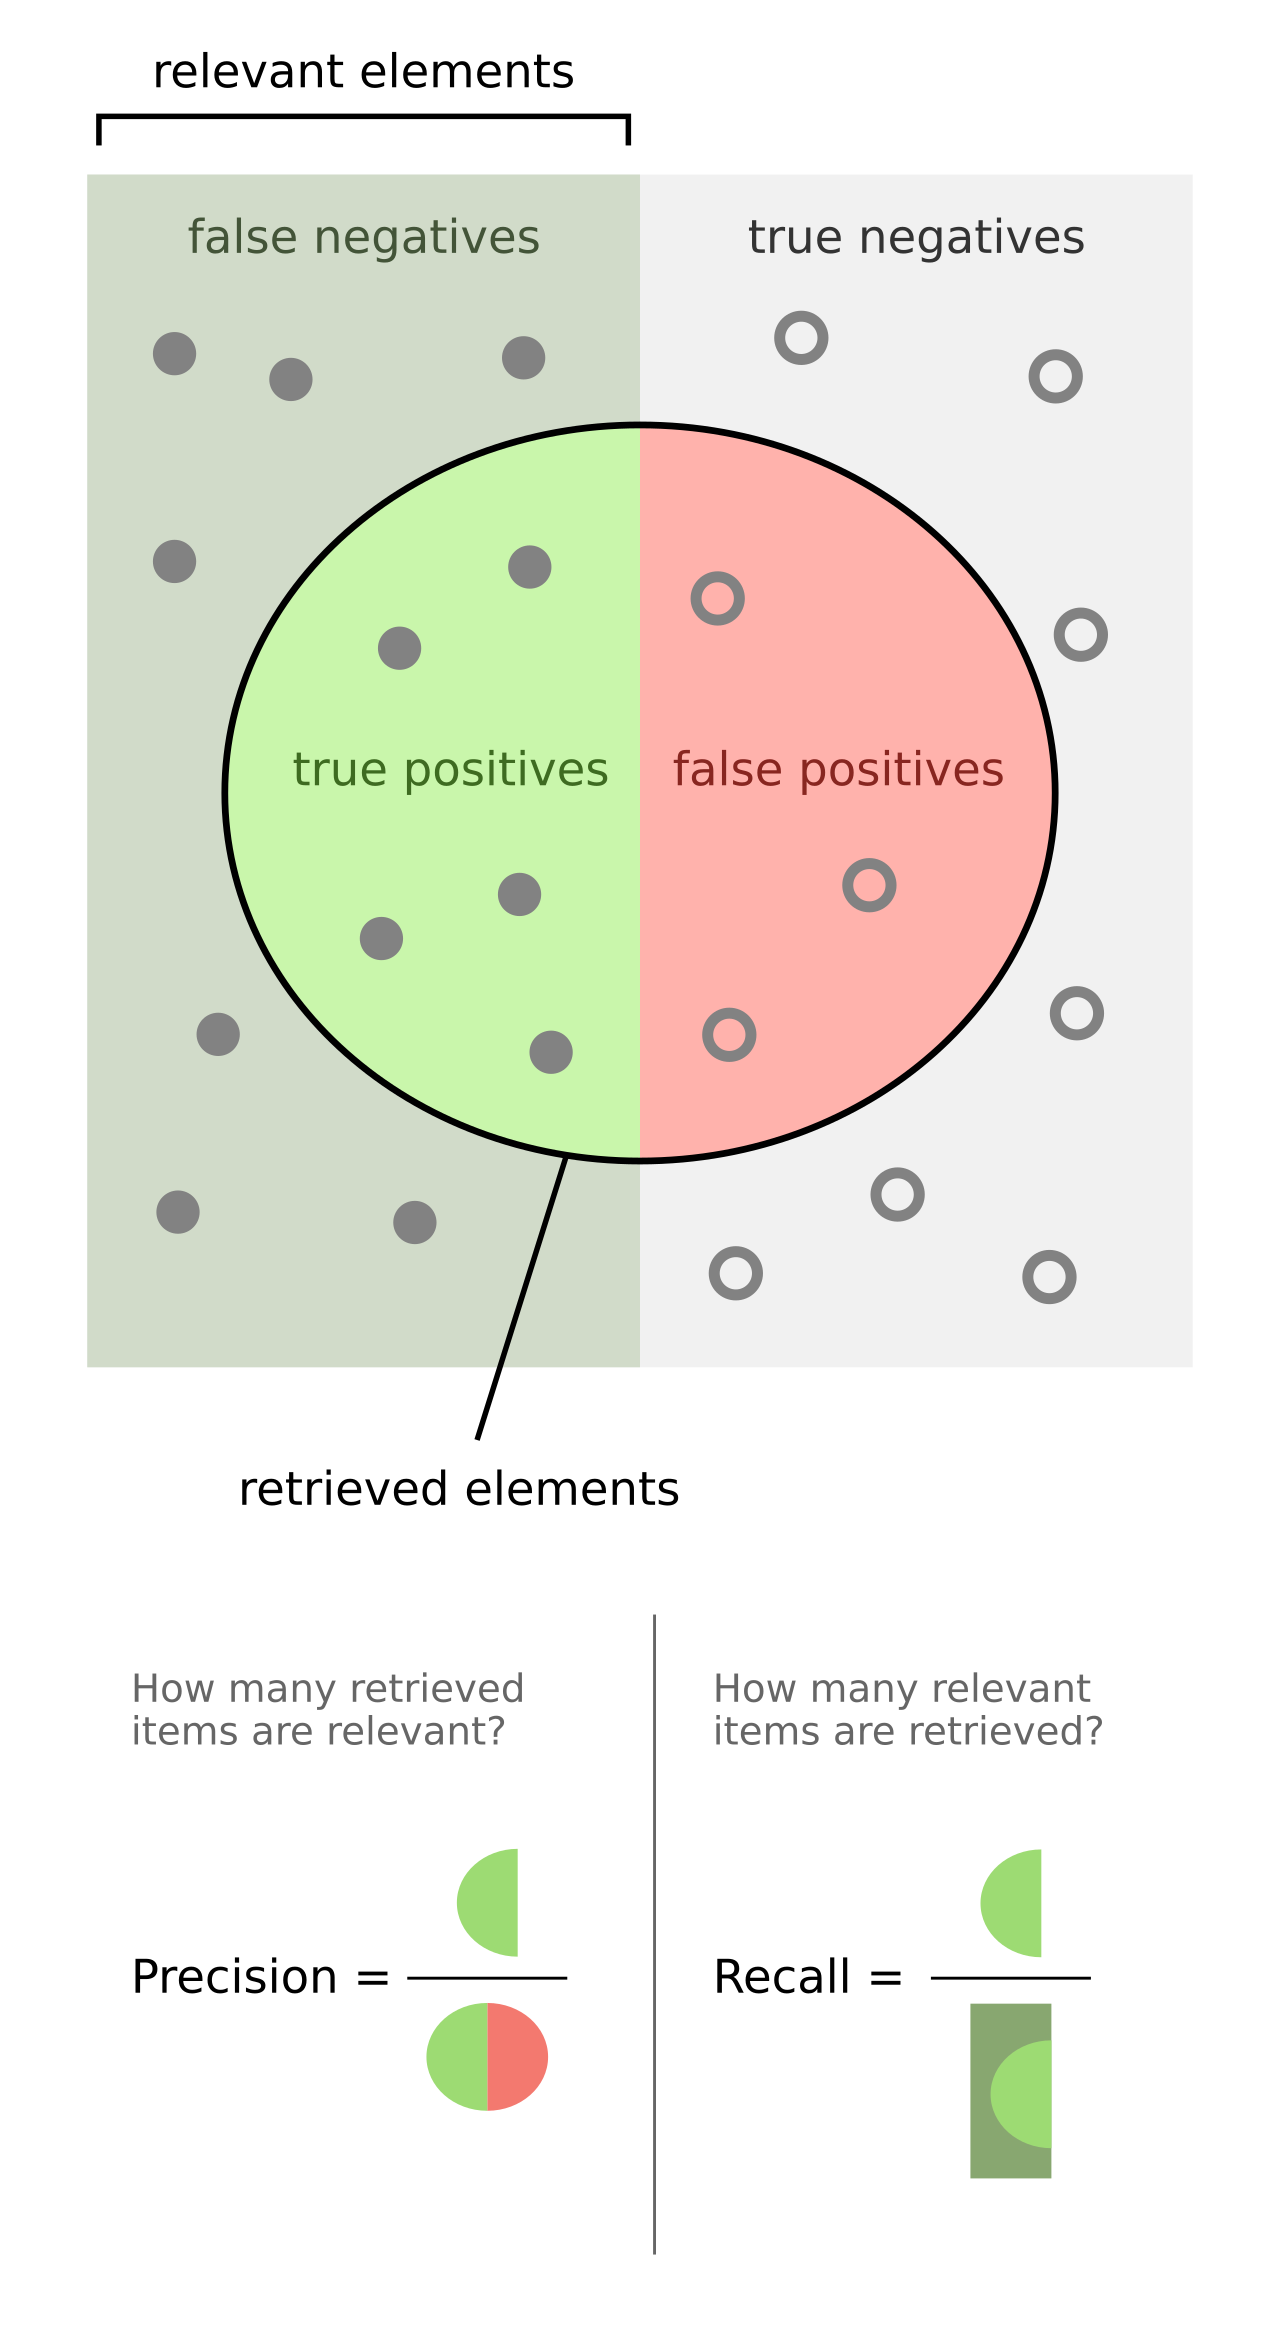
\includegraphics[width=0.56\linewidth]{assets/images/nestrukturovana-data/precision-recall.png}
  \caption[Precision a recall]{Vztah mezi precision a recall. Popis obrázku: relevantní prvky tvoří jednu
  množinu, nalezené prvky druhou; jejich průnik jsou true positives, nalezené nerelevantní prvky jsou false
  positives a nenalezené relevantní prvky jsou false negatives. Zdroj obrázku: Walber,
  \href{https://commons.wikimedia.org/wiki/File:Precisionrecall.svg}{Wikimedia Commons}, licence CC BY-SA 4.0.}
  \label{fig:q17-precision-recall}
\end{figure}

\paragraph{Napětí mezi precision a recall.}
Širší dotaz často zvýší recall, ale sníží precision. Užší dotaz může zvýšit precision, ale snížit recall.

\paragraph{Poznámka k IR.}
V reálném webovém vyhledávání často neznáme všechny relevantní dokumenty, takže recall se měří obtížně.
Snáze se obvykle odhaduje precision na vrácených výsledcích.

\subsection*{Extrakce informací}

Extrakce informací, Information Extraction, převádí nestrukturovaný nebo semistrukturovaný text na
strukturovaná data.

Obecně:
\[
\text{text}
\rightarrow
\text{tabulka / databáze / znalostní graf}.
\]

Na rozdíl od Information Retrieval, kde často stačí najít relevantní dokument, se Information Extraction snaží
vytáhnout konkrétní fakta. Výstup má být dále strojově použitelný: záznam v tabulce, JSON objekt, trojice ve
znalostním grafu nebo vyplněná šablona.

Příklad:
\begin{quote}
\uv{Oliver Blume, CEO of Volkswagen, announced sales growth of 23 MEUR in 2025.}
\end{quote}

Možný strukturovaný výstup:
\[
\begin{array}{lll}
\text{entity} & \text{type} & \text{value}\\
\hline
\text{Oliver Blume} & \text{PERSON} & -\\
\text{Volkswagen} & \text{ORGANIZATION} & -\\
\text{23 MEUR} & \text{MONEY} & 23\\
\text{2025} & \text{DATE} & 2025
\end{array}
\]

A vztah:
\[
CEO\_of(\text{Oliver Blume},\text{Volkswagen}).
\]

\subsection*{Named Entity Recognition}

Named Entity Recognition, NER, hledá pojmenované entity v textu a přiřazuje jim typ.

Typické typy:
\begin{itemize}
    \item osoby,
    \item organizace,
    \item lokace a geopolitické entity,
    \item datumy,
    \item měnové částky,
    \item produkty,
    \item události,
    \item doménově specifické entity.
\end{itemize}

Přístupy k NER:
\begin{itemize}
    \item \textbf{regulární výrazy} -- vhodné pro formální entity, například částky nebo data;
    \item \textbf{gazetteery} -- slovníky známých entit;
    \item \textbf{ručně psaná pravidla} -- využívají kontext, tvar slov a gramatiku;
    \item \textbf{statistické modely} -- například CRF;
    \item \textbf{transformerové modely a LLM} -- dnes velmi silné pro mnoho jazyků a domén.
\end{itemize}

\paragraph{Problém gazetteerů.}
Slovník entit může říct, že \uv{Denver} je město, ale v konkrétním textu může jít o osobu. Naopak nová firma
nebo produkt ještě ve slovníku nemusí být.

\subsection*{Entity linking}

Entity linking nejde jen po typu entity, ale po konkrétní entitě ve znalostní bázi:
\[
\text{\uv{Paris}}
\rightarrow
\text{Paris, France}
\quad
\text{nebo}
\quad
\text{Paris Hilton}.
\]

Postup:
\begin{enumerate}
    \item rozpoznat kandidátní entitu v textu,
    \item najít kandidáty ve znalostní bázi,
    \item vybrat správnou entitu podle kontextu,
    \item propojit text s identifikátorem ve znalostním grafu.
\end{enumerate}

Příklady znalostních bází:
\begin{itemize}
    \item Wikidata,
    \item DBpedia,
    \item YAGO,
    \item interní firemní znalostní graf.
\end{itemize}

\subsection*{Relation extraction}

Relation extraction hledá vztahy mezi entitami:
\[
relation(entity_1,entity_2).
\]

Příklady:
\[
works\_for(\text{person},\text{organization}),
\]
\[
located\_in(\text{company},\text{country}),
\]
\[
acquired(\text{company}_1,\text{company}_2).
\]

Přístupy:
\begin{itemize}
    \item pravidla a vzory,
    \item dependency parsing,
    \item supervised learning,
    \item distant supervision,
    \item transformerové modely,
    \item LLM s kontrolou výstupu.
\end{itemize}

\subsection*{Web scraping}

Web scraping je automatizované získávání dat z webových stránek. Cílem je převést webový obsah na
strukturovaná data:
\[
HTML
\rightarrow
\text{tabulka / JSON / databáze}.
\]

\begin{figure}[htbp]
  \centering
  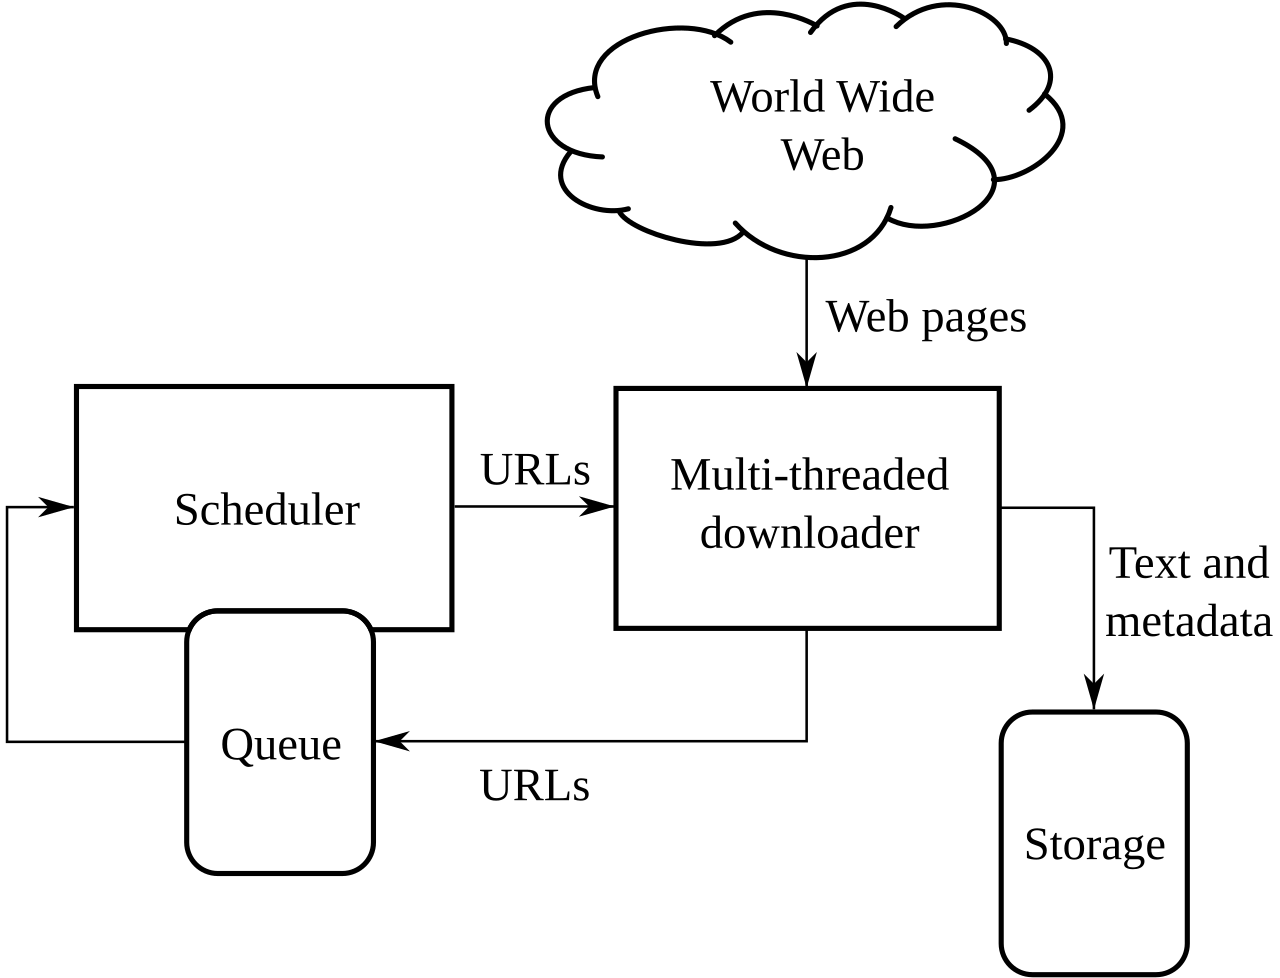
\includegraphics[width=0.86\linewidth]{assets/images/nestrukturovana-data/web-crawler-architecture.png}
  \caption[Architektura webového crawleru]{Základní architektura webového crawleru. Popis obrázku: scheduler
  spravuje frontu URL, downloader stahuje webové stránky a z textu, metadat a odkazů se doplňuje další obsah
  nebo nové URL do fronty. Zdroj obrázku: dnet podle ChaTo,
  \href{https://commons.wikimedia.org/wiki/File:WebCrawlerArchitecture.svg}{Wikimedia Commons}, licence
  CC BY-SA 3.0.}
  \label{fig:q17-web-crawler}
\end{figure}

\paragraph{Crawler vs. scraper.}
Crawler systematicky prochází odkazy a objevuje stránky. Scraper z konkrétních stránek extrahuje požadované
položky. V praxi se oba kroky často kombinují: crawler najde stránky a scraper z nich vytáhne strukturovaná
data.

\subsection*{API vs. scraping}

\begin{itemize}
    \item \textbf{API} poskytuje data ve strukturované podobě, typicky JSON nebo XML.
    Je stabilnější a vhodnější, pokud existuje.
    
    \item \textbf{Scraping} získává data přímo z HTML stránky. Je křehčí, protože změna vzhledu stránky může
    rozbít extrakční pravidla.
\end{itemize}

Obecně:
\[
\text{API} > \text{scraping},
\]
pokud API poskytuje potřebná data, je dostupné a jeho podmínky umožňují použití.

\subsection*{Typický postup web scrapingu}

\begin{enumerate}
    \item definovat cíl a datové položky,
    \item ověřit dostupnost API,
    \item zkontrolovat podmínky použití webu,
    \item stáhnout stránku přes HTTP požadavek,
    \item naparsovat HTML do DOM stromu,
    \item vybrat prvky pomocí CSS selektorů nebo XPath,
    \item zpracovat paginaci nebo odkazy,
    \item vyčistit a normalizovat data,
    \item uložit výstup do CSV, JSON, databáze nebo datového skladu,
    \item monitorovat změny struktury webu.
\end{enumerate}

HTTP požadavek:
\[
GET\ /products?page=1
\]

Výstup:
\[
\texttt{status code},\quad \texttt{headers},\quad \texttt{body}.
\]

\subsection*{CSS selektory a XPath}

CSS selektor:
\[
\texttt{div.product span.price}
\]

XPath:
\[
\texttt{//div[@class='product']//span[@class='price']}
\]

CSS selektory bývají jednodušší, XPath je expresivnější pro složitější stromové dotazy.

\subsection*{Dynamické weby}

Mnoho webů načítá obsah pomocí JavaScriptu. Pak jednoduché stažení HTML nemusí stačit.

Možnosti:
\begin{itemize}
    \item najít síťový API požadavek v prohlížeči,
    \item použít headless browser,
    \item použít Selenium nebo Playwright,
    \item počkat na vykreslení stránky,
    \item zpracovat infinite scroll.
\end{itemize}

\subsection*{Wrapper generation}

Wrapper je extrakční pravidlo nebo program, který z daného typu stránky vytahuje požadovaná data.

Příklad:
\[
\text{produktová stránka}
\rightarrow
\{\text{název},\text{cena},\text{dostupnost},\text{hodnocení}\}.
\]

Wrapper může být:
\begin{itemize}
    \item ručně napsaný,
    \item interaktivně vytvořený klikáním na prvky ve stránce,
    \item částečně automaticky naučený z příkladů.
\end{itemize}

Výhoda wrapperu:
\begin{itemize}
    \item vysoká přesnost pro konkrétní web.
\end{itemize}

Nevýhoda:
\begin{itemize}
    \item křehkost při změně šablony webu.
\end{itemize}

\subsection*{Právní a etické aspekty scrapingu}

Při scrapingu je nutné řešit:
\begin{itemize}
    \item podmínky použití webu,
    \item soubor \texttt{robots.txt},
    \item autorská práva a databázová práva,
    \item ochranu osobních údajů,
    \item zákaz obcházení technických omezení,
    \item přiměřenou zátěž serveru,
    \item transparentnost účelu sběru dat.
\end{itemize}

\paragraph{Robots.txt.}
Soubor \texttt{robots.txt} říká crawlerům, které části webu nemají navštěvovat. Není to totéž co právní
smlouva, ale je to důležitá technická a etická konvence.

\paragraph{Rate limiting.}
Slušný scraper omezuje frekvenci požadavků, používá cache, identifikuje se rozumným user-agentem a respektuje
chyby serveru. Technicky funkční scraping ještě neznamená, že je vhodný právně, eticky nebo provozně.

\paragraph{Osobní údaje.}
Pokud scraping získává osobní údaje, je nutné mít právní titul zpracování, minimalizovat rozsah dat,
zajistit bezpečné uložení a respektovat práva subjektů údajů.

\subsection*{Nástroje}

Pro praktickou práci se používají například:
\begin{itemize}
    \item \textbf{Python:} \texttt{requests}, \texttt{BeautifulSoup}, \texttt{lxml}, \texttt{Scrapy},
    \texttt{Selenium}, \texttt{Playwright}, \texttt{pandas};
    \item \textbf{IR a vyhledávání:} Apache Lucene, Elasticsearch, OpenSearch, Solr;
    \item \textbf{NLP/IE:} spaCy, NLTK, Stanza, UDPipe, transformers;
    \item \textbf{datové formáty:} JSON, XML, CSV, Parquet;
    \item \textbf{uložení:} relační databáze, dokumentové databáze, datové sklady, knowledge graphs.
\end{itemize}

\subsection*{Shrnutí ke zkoušce}

Nestrukturovaná a semistrukturovaná data vyžadují převod do strojově zpracovatelné podoby. Semistrukturovaná
data jako XML, JSON a HTML mají stromovou nebo dokumentovou strukturu. Nestrukturovaný text je třeba
tokenizovat, normalizovat a reprezentovat pomocí termů, vah nebo embeddingů.

Porovnávání vzorů zahrnuje regulární výrazy, edit distance a sémantickou podobnost. Vyhledávání dokumentů
využívá indexování, zejména inverted index. Booleovský model pracuje s přesnou logickou shodou, zatímco
vektorový model reprezentuje dotaz i dokument jako vektory a řadí výsledky podle podobnosti:
\[
\cos(d,q)=\frac{d^\top q}{\|d\|\|q\|}.
\]

Extrakce informací převádí text na strukturovaná data. Patří sem NER, entity linking, relation extraction a
template filling. Web scraping automatizovaně získává data z webových stránek, typicky přes HTTP, HTML DOM,
CSS selektory a XPath. Pokud existuje API, je obvykle vhodnější než scraping. Při scrapingu je nutné řešit
technická omezení, kvalitu dat, právní podmínky, etiku a ochranu osobních údajů.

\subsection*{Zdroje}

\begin{itemize}
    \item Manning, Raghavan, Schütze:
    \href{https://nlp.stanford.edu/IR-book/}{Introduction to Information Retrieval}.
    \item Python dokumentace:
    \href{https://docs.python.org/3/library/re.html}{\texttt{re} -- Regular expression operations}.
    \item MDN Web Docs:
    \href{https://developer.mozilla.org/en-US/docs/Web/API/Document\_Object\_Model}{Document Object Model}.
    \item RFC 9309:
    \href{https://www.rfc-editor.org/rfc/rfc9309}{Robots Exclusion Protocol}.
    \item Scrapy dokumentace:
    \href{https://docs.scrapy.org/en/latest/topics/selectors.html}{Selectors}.
    \item Wikimedia Commons:
    \href{https://commons.wikimedia.org/wiki/File:DOM\_Beispielbaum.svg}{DOM Beispielbaum}.
    \item Wikimedia Commons:
    \href{https://commons.wikimedia.org/wiki/File:Search-engine-diagram-en.svg}{Search-engine-diagram-en}.
    \item Wikimedia Commons:
    \href{https://commons.wikimedia.org/wiki/File:Precisionrecall.svg}{Precisionrecall}.
    \item Wikimedia Commons:
    \href{https://commons.wikimedia.org/wiki/File:WebCrawlerArchitecture.svg}{WebCrawlerArchitecture}.
\end{itemize}

\newpage
